%!TEX root = ../note.tex
% Source: ../chapter1_econ101_fall2026.pdf
\section{The four core principles of economics}
An \term{economy} is a system that answers four questions for a group of
agents facing scarce resources: \emph{what} to produce, \emph{how} to produce
it, \emph{who} does what, and \emph{who} gets what. (The slides' example is
the island in Golding's \emph{Lord of the Flies}.) The basic unit of analysis
is an \emph{individual decision}, and four principles tell us how decisions
are made:
\begin{enumerate}
  \item the cost--benefit principle,
  \item the opportunity cost principle,
  \item the marginal principle,
  \item the interdependence principle.
\end{enumerate}

\subsection{The cost--benefit principle}
Throughout, an agent chooses from a set $A$ of feasible options.

\begin{defi}
  For an option $a \in A$, let $B(a)$ be its \term{benefit} and $C(a)$ its
  \term{cost}, both measured in dollars. The \term{economic surplus} of $a$ is
  \[
    S(a) = B(a) - C(a).
  \]
\end{defi}

Benefits and costs need not be monetary. They are converted to dollars through
willingness to pay.

\begin{defi}
  The \term{willingness to pay} for a benefit is the largest amount of money
  $w$ the agent would give up to get it. For a cost, it is the largest $w$ the
  agent would pay to avoid it.
\end{defi}

\begin{principle}[Cost--benefit principle]
  Pursue an option $a$ if and only if $B(a) \geq C(a)$, i.e.\ $S(a) \geq 0$.
\end{principle}

\begin{remark}
  Some complications (the slides list them but do not resolve them yet):
  \begin{itemize}
    \item not everything is about money, which is why willingness to pay is
      used as the unit;
    \item the benefit may go to someone else;
    \item $B$ and $C$ may be uncertain, in which case they are random variables.
  \end{itemize}
  Costs and benefits are the \term{economic incentives} that drive decisions.
\end{remark}

\subsubsection*{Gains from trade}
\begin{nprop}[Voluntary exchange is not zero-sum]\label{prop:trade}
  A buyer values a good at $v$, a seller can produce it at cost $c$, and they
  trade at price $p$. Then
  \[
    S_{\text{buyer}} = v - p,\qquad S_{\text{seller}} = p - c,\qquad
    S_{\text{buyer}} + S_{\text{seller}} = v - c .
  \]
  Both agree to trade if and only if $c \leq p \leq v$, in which case both
  surpluses are nonnegative. The total surplus $v - c$ does not depend on $p$.
  The price only decides how it is split.
\end{nprop}
\begin{proof}
  The buyer accepts iff $v - p \geq 0$ and the seller accepts iff
  $p - c \geq 0$. Adding the two surpluses cancels $p$.
\end{proof}

\begin{significant}
  Voluntary exchange creates surplus $v - c \geq 0$. Nobody loses.
\end{significant}

\subsection{The opportunity cost principle}
\begin{defi}
  Given a choice $a \in A$, the \term{next best alternative} is the best
  option in $A \setminus \{a\}$. The \term{opportunity cost} of $a$ is the
  value of what is given up:
  \[
    \OC(a) = \max_{a' \in A \setminus \{a\}} (\text{value of } a').
  \]
  The out-of-pocket part of a cost is the \term{financial cost}. The
  opportunity cost can be much larger.
\end{defi}

\begin{principle}[Opportunity cost principle]
  The true cost of something is what you must give up to get it. When deciding
  on $a$, always ask ``$a$, \emph{or} the next best alternative?''
\end{principle}

Resources (income, time, energy) are \term{scarce}. That is why every choice
has an opportunity cost.

\begin{defi}
  A \term{sunk cost} is a cost that has to be paid whatever option is
  chosen, i.e.\ a cost $k$ that enters $C(a)$ for every $a \in A$.
\end{defi}

\begin{nprop}[Ignore sunk costs]\label{prop:sunk}
  If $C(a) = \tilde C(a) + k$ for all $a \in A$ with $k$ constant, then
  \[
    \argmax_{a \in A} \bigl(B(a) - C(a)\bigr) = \argmax_{a \in A} \bigl(B(a) - \tilde C(a)\bigr).
  \]
\end{nprop}
\begin{proof}
  Subtracting the constant $k$ from every surplus preserves their order.
\end{proof}

\begin{eg}
  Tuition is \dollar{4{,}500} per term for 5 courses with 24 lectures each, so
  one lecture costs $\frac{4500}{5 \cdot 24} = \dollar{37.50}$. You pay this
  whether you attend or not, so it is sunk and does not affect the decision.
  The relevant cost of going to lecture is the next best use of those 80
  minutes, e.g.\ wages from a job.
\end{eg}

\begin{eg}
  The biggest cost of an hour of gaming is not the hardware or software. It is
  the hour, which could have been spent on something else.
\end{eg}

\begin{ex}
  Explain each of the following with the opportunity cost principle.
  \begin{enumerate}
    \item Many Canadians date as teenagers but few marry as teenagers.
    \item There are fewer stay-at-home mothers than 60 years ago.
    \item More Canadians are born in September--October than in February--March.
    \item Terminally ill patients are more willing to try unproven drugs.
  \end{enumerate}
\end{ex}
\begin{remark}[Sketch]
  In (ii), higher wages for women raise the opportunity cost of staying at
  home. In (iv), the patient gives up fewer expected years of life, so the
  opportunity cost of the risk is lower.
\end{remark}

\subsubsection*{Production possibilities frontier}
\begin{defi}
  Given scarce resources, the \term{feasible set} $F \subseteq \R_{\geq 0}^2$ is
  the set of output pairs $(x, y)$ that can be produced. A point
  $(x, y) \in F$ is \term{efficient} if there is no $(x', y') \in F$ with
  $x' \geq x$, $y' \geq y$ and $(x', y') \neq (x, y)$. The
  \term{production possibilities frontier} (PPF) is the set of efficient
  points in $F$.
\end{defi}

On a PPF $y = f(x)$ with $f$ decreasing, the opportunity cost of one more
unit of $x$ is the amount of $y$ given up, $-\Delta y / \Delta x$. For a
differentiable $f$ this is $\abs{f'(x)}$, the absolute value of the slope.

\begin{eg}[Studying]\label{eg:ppf}
  You have $3$ hours a night for economics ($h_e$) and psychology ($h_p$), so
  $h_e + h_p \leq 3$. Each hour raises your economics grade by $8$ points and
  your psychology grade by $4$ points:
  \[
    E = 8h_e,\qquad P = 4h_p.
  \]
  Substituting $h_e = E/8$ and $h_p = P/4$ gives
  \[
    F = \set{(P, E) \in \R_{\geq 0}^2 : \tfrac{E}{8} + \tfrac{P}{4} \leq 3},
    \qquad \text{PPF: } E = 24 - 2P,\quad 0 \leq P \leq 12.
  \]
  The opportunity cost of one psychology point is $2$ economics points. For
  example, going from $(4, 16)$ to $(8, 8)$ costs $8$ economics points for
  $4$ psychology points. Points strictly inside $F$, such as $(3, 10)$, are
  \emph{inefficient}.
\end{eg}

\begin{center}
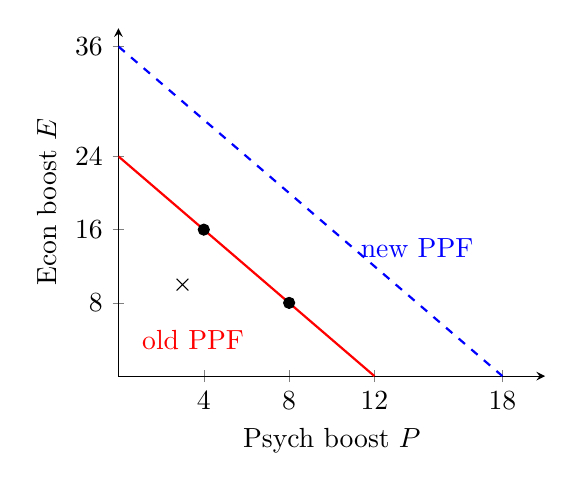
\begin{tikzpicture}
  \begin{axis}[width=7cm, height=6cm, xmin=0, xmax=20, ymin=0, ymax=38,
      xlabel={Psych boost $P$}, ylabel={Econ boost $E$},
      axis lines=left, xtick={4,8,12,18}, ytick={8,16,24,36}]
    \addplot[thick, red, domain=0:12] {24 - 2*x};
    \addplot[thick, blue, dashed, domain=0:18] {36 - 2*x};
    \addplot[only marks, mark=*] coordinates {(4,16) (8,8)};
    \addplot[only marks, mark=x, mark size=3pt] coordinates {(3,10)};
    \node[red] at (axis cs:3.5,4) {old PPF};
    \node[blue] at (axis cs:14,14) {new PPF};
  \end{axis}
\end{tikzpicture}
\end{center}

\begin{nprop}[Features of a PPF]
  \leavevmode
  \begin{enumerate}
    \item Every point on the PPF is efficient: one output can only be raised
      by lowering the other.
    \item The absolute value of the slope of the PPF is the opportunity cost
      of the good on the horizontal axis.
    \item Higher productivity enlarges $F$ and pushes the PPF outward.
  \end{enumerate}
\end{nprop}

\begin{eg}
  In Example~\ref{eg:ppf}, suppose productivity rises by $50\%$ in both
  subjects: $E = 12h_e$ and $P = 6h_p$. The new PPF is $E = 36 - 2P$ for
  $0 \leq P \leq 18$. The frontier moves out, but the opportunity cost is
  still $12/6 = 2$.
\end{eg}

\subsection{The marginal principle}
So far choices were binary. Many choices are about \emph{how much}: choose a
quantity $q \in \set{0, 1, 2, \ldots}$.

\begin{defi}
  Let $\TB(q)$ and $\TC(q)$ be the \term{total benefit} and \term{total cost}
  of quantity $q$. For $q \geq 1$ the \term{marginal benefit} and
  \term{marginal cost} of the $q$-th unit are
  \[
    \MB(q) = \TB(q) - \TB(q-1),\qquad \MC(q) = \TC(q) - \TC(q-1).
  \]
  The surplus is $S(q) = \TB(q) - \TC(q)$.
\end{defi}

\begin{principle}[Marginal principle]
  Break a decision about quantity into a sequence of marginal decisions:
  ``should I get one more?'' Answer each one with the cost--benefit
  principle, i.e.\ compare $\MB(q+1)$ with $\MC(q+1)$.
\end{principle}

\begin{nlemma}\label{lem:telescope}
  For all $q \geq 0$,
  \[
    S(q) = S(0) + \sum_{k=1}^{q} \bigl(\MB(k) - \MC(k)\bigr).
  \]
\end{nlemma}
\begin{proof}
  The sum telescopes:
  $\sum_{k=1}^q \MB(k) = \TB(q) - \TB(0)$, and similarly for $\MC$.
\end{proof}

\begin{nthm}[Rational rule]\label{thm:rational}
  Suppose $\MB - \MC$ is nonincreasing (this holds, for instance, if $\MB$
  is nonincreasing and $\MC$ is nondecreasing). Then
  \[
    q^* = \max\set{q \geq 0 : q = 0 \text{ or } \MB(q) \geq \MC(q)}
  \]
  maximises $S$. In words: \emph{keep going as long as the marginal benefit
  is at least the marginal cost.}
\end{nthm}
\begin{proof}
  Write $d(k) = \MB(k) - \MC(k)$, which is nonincreasing. By the choice of
  $q^*$ and monotonicity, $d(k) \geq 0$ for $k \leq q^*$ and $d(k) < 0$ for
  $k > q^*$. By Lemma~\ref{lem:telescope}, if $q < q^*$ then
  $S(q^*) - S(q) = \sum_{k=q+1}^{q^*} d(k) \geq 0$, and if $q > q^*$ then
  $S(q) - S(q^*) = \sum_{k=q^*+1}^{q} d(k) < 0$.
\end{proof}

\begin{remark}
  If $q$ can vary continuously and $\TB$, $\TC$ are differentiable, then
  $\MB = \TB'$ and $\MC = \TC'$. An interior optimum satisfies the
  first-order condition $S'(q^*) = 0$, i.e.
  \[
    \MB(q^*) = \MC(q^*).
  \]
  It is a maximum when $S'' = \MB' - \MC' \leq 0$. This is the
  ``marginal benefit equals marginal cost'' form of the rule.
\end{remark}

\begin{eg}[Nerida's restaurant]
  Each meal sells for \dollar{25}. Total cost is \dollar{10} per meal in food,
  \dollar{300} per waiter, \dollar{500} rent, and \dollar{1{,}000} for
  Nerida's own time. How many waiters should she hire?
  \begin{center}
    \begin{tabular}{ccccccc}
      \toprule
      Workers & Meals & $\TB$ & $\MB$ & $\TC$ & $\MC$ & $S$ \\
      \midrule
      2 & 160 & 4000 & ---  & 3700 & --- & 300 \\
      3 & 210 & 5250 & 1250 & 4500 & 800 & 750 \\
      4 & 250 & 6250 & 1000 & 5200 & 700 & 1050 \\
      5 & 280 & 7000 & 750  & 5800 & 600 & 1200 \\
      6 & 300 & 7500 & 500  & 6300 & 500 & \textbf{1200} \\
      7 & 310 & 7750 & 250  & 6700 & 400 & 1050 \\
      \bottomrule
    \end{tabular}
  \end{center}
  For example, the 4th worker adds $40$ meals, so
  $\MB(4) = 25 \cdot 40 = 1000$ and $\MC(4) = 300 + 10 \cdot 40 = 700$.
  Here both $\MB$ and $\MC$ fall, but $\MB - \MC = 450, 300, 150, 0, -150$
  is still decreasing, so Theorem~\ref{thm:rational} applies. The
  rule stops at $q^* = 6$, where $\MB = \MC = 500$, and the maximum surplus is
  \dollar{1{,}200}. (The 6th worker adds exactly zero surplus, so $q = 5$ is
  also optimal.)
\end{eg}

\begin{remark}
  Rent and Nerida's time are the same for every $q$. They are sunk with
  respect to this decision and never appear in $\MC$
  (Proposition~\ref{prop:sunk}).
\end{remark}

\subsection{The interdependence principle}
\begin{principle}[Interdependence principle]
  Your best choice in one situation depends on:
  \begin{enumerate}
    \item \emph{your other choices}: resources (income, time, attention,
      wealth) are shared across all your decisions;
    \item \emph{other people's choices}: scarcity creates competition between
      agents (people, businesses, governments);
    \item \emph{other markets}: e.g.\ labour, housing and credit markets affect
      one another;
    \item \emph{time}: today's choice depends on past choices and expected
      future ones.
  \end{enumerate}
\end{principle}

\begin{remark}
  Mathematically, (i) says you solve one problem subject to a joint budget
  constraint (as in the PPF), not several problems separately. Points (ii) and
  (iii) say that the parameters of your problem, such as prices, are
  determined by the choices of everyone else.
\end{remark}
